\documentclass{article}

\usepackage[top=1in,bottom=1in,left=1in,right=1in]{geometry}
\usepackage{graphicx}

\title{MAEbot Datasheet}
\author{EECS 467}

\begin{document}

\maketitle

\begin{table}[h]
\caption{Units}
\centering
\begin{tabular}{| r | l  l |}
\multicolumn{2}{r}{} \\  % put this here to get rid of the vertical lines, but the caption is otherwise too close
\hline
\textbf{Distance:}         & meters         & $m$      \\
\hline
\textbf{Linear Velocity:}  & meters/second  & $m/s$    \\
\hline
\textbf{Orientation:}      & radians        & $rad$     \\
\hline
\textbf{Angular Velocity:} & radians/second & $rad/s$   \\
\hline
\end{tabular}
\end{table}

\begin{table}[h]
\caption{Robot Parameters}
\centering
\begin{tabular}{| r | l |}
\multicolumn{2}{r}{} \\  % put this here to get rid of the vertical lines, but the caption is otherwise too close
\hline
\textbf{Ticks/Rev:}       & 480     \\
\hline
\textbf{Wheel Diameter:}  & 0.032m  \\
\hline
\textbf{Wheelbase:}       & 0.08m   \\
\hline
\end{tabular}
\end{table}

\begin{figure}[h]
\begin{center}
 \includegraphics{./maebot_frame.png}
 \caption{The MAEbot reference frame uses a right-handed coordinate system. The robot drives forward along the x-axis. Positive angles are to the left of the robot, negative 
          angles to the right.}
\end{center}
\end{figure}


\section*{Connecting to the MAEbot}

Each team has an account on every MAEbot.

\begin{description}
  \item[\textbf{User:}]     teamN   (where N is your assigned team number)
  \item[\textbf{Password:}] eecs467
\end{description}
  

This setup allows you to easily switch between robots if your battery dies or something else is wrong with your robot. You can simply pull your repository into your home directory 
on the new robot and off you go!

There are two ways we've been connecting to the MAEBots:

\begin{itemize}
 \item Plug-In Console
 \item SSH over 802.11 WiFi
\end{itemize}

\subsection*{Plug-In Console}
Plug a usb mini cable into the console port on the top board and execute:

\begin{verbatim}
  screen /dev/ttyUSBX 115200
\end{verbatim}

You can also watch the whole boot sequence on this port, which can be useful for debugging. Though hopefully you won't need to debug anything in the boot process.
Be careful with this cable. If you trip over it, you can pull the connector off the board, which will require your robot to be sent off to the repair shop to resolder it.

\subsection*{SSH over WiFi}
The MAEBots are programmed to connect to an open network named "maenet2", configured on the 192.168.3 network. Each robot will connect with an IP address of 192.168.3.XXX, where XXX is based on the robot's serial number. The 
serial numbers are written on the top and bottom of each robot. You can connect via Wifi with the command:

\begin{verbatim}
For S/N [1-9]:
  ssh teamN@192.168.3.10{S/N}

For S/N [10-14]:
  ssh teamN@192.168.3.1{S/N}

\end{verbatim}

\end{document}

